\documentclass{exam}
\pagestyle{headandfoot}
\firstpageheadrule
\runningheadrule
\firstpageheader{CT - Topic 1}{}{Sam Robbins}
\runningheader{CT - Topic 1}{What is computer hardware}{Sam Robbins}
\firstpagefooter{}{}{}
\runningfooter{}{}{}
\renewcommand{\solutiontitle}{\noindent\textbf{Solution:}\par\noindent}


\printanswers
\usepackage{graphicx}
\marksnotpoints
\bracketedpoints
\pointsdroppedatright
\pointsinrightmargin
\begin{document}
\begin{center}
	\underline{\huge What is computer hardware?}
\end{center}
\begin{questions}
\question[3] What are the three fundamental phases of integrated circuit design?
You should briefly explain what each phase does. 

\begin{solution}[.2in]
A \textbf{functional specification} $[\frac{1}{2}]$ of the chip is derived (this describes
exactly what the IC is supposed to do involving factors like chip area,
power, speed and cost $[\frac{1}{2}]$); the \textbf{register transfer level (RTL)} $[\frac{1}{2}]$ design
is then undertaken (the functional specification is used to describe
the exact behaviour of the digital circuits on the chip, as well as the
interconnections to inputs and outputs, with this description being in
terms of logic gates and interconnecting wires $[\frac{1}{2}]$); and then the RTL
design is \textbf{mapped to a physical layout} $[\frac{1}{2}]$ in silicon (specific physical
attributes must be respected; for example, it is crucial that appropriate
spacing between transistors is maintained in the physical layout $[\frac{1}{2}]$).
\end{solution}

\question[10] What is a NAND-gate? Show how a NOT-gate, an AND-gate and an
OR-gate can be constructed using just NAND-gates
\begin{solution}[.2in]
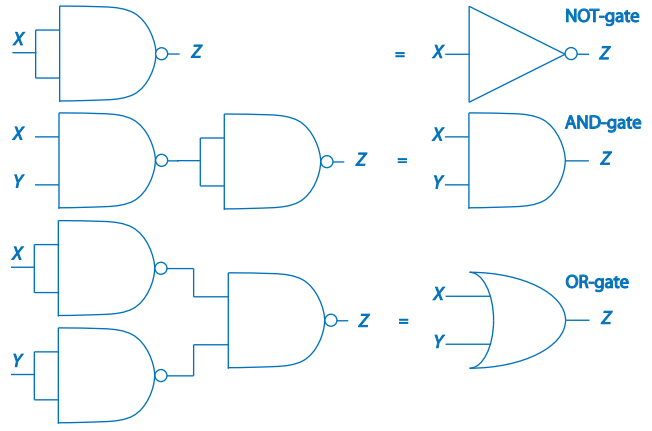
\includegraphics[width=8cm]{NAND.png}
\end{solution}
\newpage
\question[6]Build a circuit using NOT-, AND- and OR-gates that computes the
function with 3 Boolean inputs and where the output is 1 if, and only
if, there are an even number of 1’s in the input.
\begin{solution}[.2in]
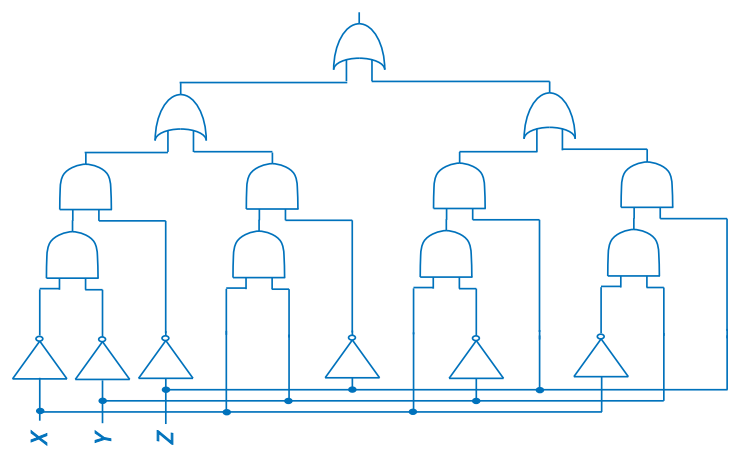
\includegraphics[width=11cm]{even.png}
\end{solution}
\question[7]What are a half-adder and a full-adder? Show how a full-adder can be
built using 2 half-adders
\begin{solution}[.2in]
A half-adder takes x and y as inputs and computes the Boolean sum
of x and y, where the Boolean sum of a collection of inputs is 1 if, and
only if, an odd number of the inputs are 1, and also the resulting carry
bit, which is 1 if, and only if, both x and y are 1 [2]. A full-adder takes
x, y, and z as inputs and computes the Boolean sum of x, y, and z,
resulting in the sum-bit and the carry-bit [2].\\
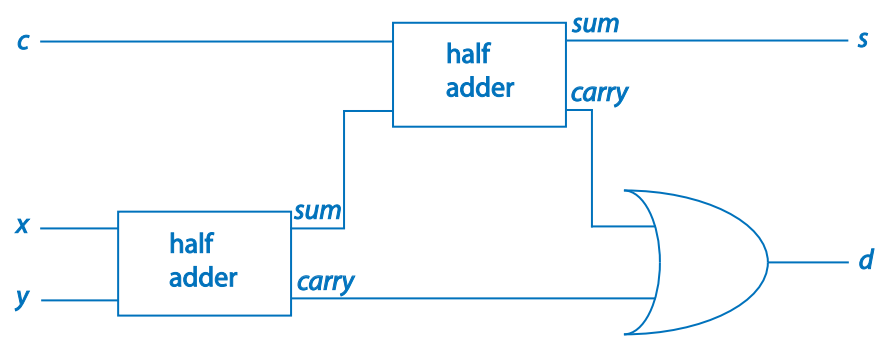
\includegraphics[width=8cm]{full_adder.png}
\end{solution}
\question[3]Name three key components in a CPU microarchitecture and briefly
describe the purpose of each.
\begin{solution}[.2in]
The \textbf{datapath} $[\frac{1}{2}]$ performs all the data processing operations and includes
the arithmetic logic unit (ALU), which is the part of the CPU
that performs all the arithmetic and logical operations on data, and a
limited number of memory locations called registers $[\frac{1}{2}]$. The \textbf{control}
$[\frac{1}{2}]$ tells the datapath, memory and input/output (I/O) devices what
to do (it is the conduit between the datapath and the main memory) $[\frac{1}{2}]$. A \textbf{cache} $[\frac{1}{2}]$ consists of small, fast and relatively expensive on-chip
memory and is used to store memory items that need to be regularly
accessed $[\frac{1}{2}]$.
\end{solution}
\newpage
\question[6]Name two types of bus within a CPU and explain the general purpose
of each. What is the width of a bus? Explain how the width of a bus
imposes memory or data limitations within a CPU.
\begin{solution}[.2in]
	Buses include a \textbf{data bus} $[\frac{1}{2}]$, an \textbf{address bus} $[\frac{1}{2}]$ and a \textbf{control bus} $[\frac{1}{2}]$. A data bus carries the contents of memory locations between the
	processor and main memory $[\frac{1}{2}]$. The address bus holds addresses of
	locations in main memory $[\frac{1}{2}]$. The control bus is used to transfer
	information between the CPU and various other devices within the
	processor $[\frac{1}{2}]$. The width of a bus is the number of parallel wires in
	a bus [1]. The width of the data bus determines the word-size of the
	computer [1]. The width of an address bus determines the size of
	addressable memory [1].
\end{solution}

\question[5]Explain carefully the four phases of the fetch-decode-fetch-execute processor cycle (be sure to explain the purpose of any CPU components
you happen to mention).
\begin{solution}[.2in]
The ‘\textbf{instruction fetch}’ phase involves the supply of the instruction address
(via the address bus) and the return from memory (via the data
bus) of the instruction [1]. The ‘\textbf{instruction decode}’ phase involves
interpreting the stored instruction within the CPU [1]. The ‘\textbf{operand
	fetch}’ phase involves the supply of the address of any required data (via
the address bus) and the return from memory (via the data bus) of this
data [1]. The ‘\textbf{execute instruction}’ phase involves the CPU performing
the necessary actions [1] (this phase is sometimes split into two with
the ‘execute instruction’ phase followed by a ‘write-back’ phase where
data is written back to memory, if needs be [1]).
\end{solution}

\question[4]Show different layers of abstraction in a modern computer system.
\begin{solution}[.2in]
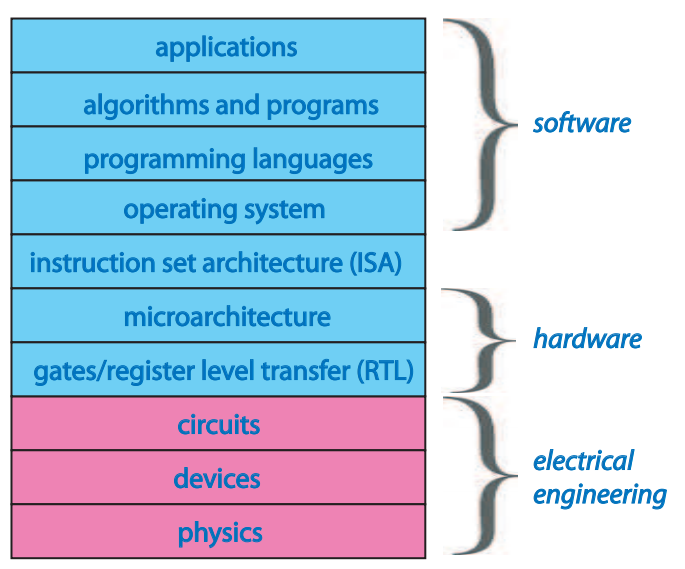
\includegraphics[width=8cm]{CSys.png}
\end{solution}
\newpage
\question[2]In a PC, there tend to be two chip-sets: the northbridge; and the
southbridge. What is the essential difference between the two?
\begin{solution}[.2in]
The northbridge handles fast communications amongst the CPU, the
memory and the graphics processing unit [1], whereas the southbridge
handles (slower) communications involving external hard-disks, the
mouse, the keyboard, the Internet, the printer and other such devices
[1].
\end{solution}

\question[1]What are the two main components of an integrated circuit? (Both of
these components usually appear in their millions.)
\begin{solution}[.2in]
Transistors [$\frac{1}{2}$] interconnected by microscopic wires [$\frac{1}{2}$].
\end{solution}

\question[2]What is the current trend in microprocessor design so as to overcome
difficulties with power dissipation as we build faster and faster single
processors?
\begin{solution}[.2in]
Multi-core processors [1] where one CPU with a high clock-speed is
replaced with a number of CPUs with lower clock-speeds but which,
when working together, can give better computational power [1].
\end{solution}

\question[1]What is Moore’s Law?
\begin{solution}[.2in]
A rough description that long-term transistor capacity doubles every
18–24 months (coined by Gordon Moore in 1965) [1].
\end{solution}

\question[2]What is a Boolean function? In relation to Boolean functions, what is
so special about NOT-, AND- and OR-gates?
\begin{solution}[.2in]
A Boolean function is a function $f:\{0, 1\}^n \rightarrow \{0, 1\}$ [1]. We can build
a circuit to compute any Boolean function using only NOT-, AND- and
OR-gates [1].
\end{solution}
\newpage
\question[6]Explain the basic principle behind using half-adders and full-adders to
build a circuit that computes the sum of two n-bit strings of 0s and 1s.
(You need not describe the resulting circuit in full detail; just give an
overview of its construction.)
\begin{solution}[.2in]
{\small Let the two n-bit strings be $X_1X_2 ... X_n$ and $Y_1Y_2 . . . Y_n$. A half-adder
	takes $X_1$ and $Y_1$ as input and outputs the sum, with the carry fed into
	a full-adder [2]. This full-adder also has inputs $X_2$ and $Y_2$ and its sum
	is output, with its carry fed into a full-adder [2]. This full-adder also
	has $X_3$ and $Y_3$ as inputs and its sum is output, with its carry fed into
	a full-adder, and so on [2]. Both the sum and the carry of the final
	full-adder are output.}
\end{solution}

\question[1]What is the ultimate aim of research in formal methods?
\begin{solution}[.2in]
The ultimate aim of formal methods is to enable us to mathematically
prove properties of designs, programs and so on, so as not just to rely
on empirical testing [1].
\end{solution}

\question[2]A hardware description language is used so as to better enable the
design of integrated circuits. Name two distinctive attributes of computer
hardware that are normally expressible in a hardware description
language.
\begin{solution}[.2in]
Unlike a normal programming language, an HDL includes explicit notations
for expressing \textbf{time} [1] and \textbf{concurrency} [1], which are primary
attributes of computer hardware
\end{solution}

\question[3]What is the von Neumann bottleneck? Which component of a modern
CPU did the von Neumann bottleneck give rise to?
\begin{solution}[.2in]
The von Neumann bottleneck is a limitation of the rate of data transfer
between the CPU and memory (data and instructions have to be
fetched in sequential order and idle time is wasted whilst waiting for
data items or instructions to be fetched from memory) [2]. The von
Neumann bottleneck gave rise to the use of caches [1].
\end{solution}


\question[2]How does the Harvard architecture differ from the von Neumann architecture?
\begin{solution}[.2in]
The Harvard architecture has memory that is partitioned into data
memory and instruction memory with dedicated buses for each of them
[2].
\end{solution}
\newpage
\question[1]What is a basic principle as regards different types of memory and its physical distance from the CPU?
\begin{solution}[.2in]
The cost and performance of memory is generally proportional to its
physical distance from the CPU [1].
\end{solution}

\question[3]What is the difference between static RAM and dynamic RAM?
\begin{solution}[.2in]
Dynamic RAM (DRAM) is where a bit of data is stored using a transistor/capacitor
combination [1]. Static RAM (SRAM) is where a bit
of data is stored by a flip-flop, which incorporates 4-6 transistors [1].
Static RAM is stable and fast but takes up more memory $[\frac{1}{2}]$ whereas
dynamic RAM is cheap, slow and needs to be refreshed because of
‘leaky’ capacitors $[\frac{1}{2}]$.
\end{solution}


\question[1]What is the purpose of cache memory in a CPU?
\begin{solution}[.2in]
Caches are expensive memory that are used to store rapidly accessed
items [1].
\end{solution}

\question[1]What are registers in the CPU?
\begin{solution}[.2in]
Registers are on-chip memory locations that are limited in number.
They provide the fastest way to access data [1].
\end{solution}

\question[2]Give two illustrations of principles of Computational Thinking in the context of hardware
\begin{solution}[.2in]
	‘Processing in parallel’ in multi-core or GPGPU computing. ‘Using
	abstraction and decomposition in tackling a large complex task’ in IC
	design and computer system design. ‘Prefetching and caching in anticipation
	of future use’ in caching within CPUs. ‘Interpreting code as data
	and data as code’ in processor architectures. [1] for each illustration.
\end{solution}





\end{questions}



\end{document}